\documentclass[a4paper,12pt]{article}
\usepackage{amssymb}
\usepackage{amsfonts}
\usepackage{amsthm}
\usepackage{amsmath}
\usepackage[T1]{fontenc}
\usepackage[utf8]{inputenc}
\usepackage[british]{babel}
\usepackage{times}
\usepackage{anysize}
\usepackage{color}
\usepackage{listings}
\usepackage{graphicx}
\usepackage{enumerate}
\usepackage{multicol}
\usepackage{float}

\usepackage{lmodern}  % for bold teletype font
\usepackage{xcolor}   % for \textcolor
%\lstloadlanguages{matlab}
\lstset{
	basicstyle=\ttfamily,
	columns=fullflexible,
%	frame=single,
	breaklines=true,
	postbreak=\mbox{\textcolor{red}{$\hookrightarrow$}\space},
}

\begin{document}
\begin{titlepage}
\center
\vspace*{\fill}
\Huge{Modeling of Physical Systems}\\
\Large{Heat transfer simulation}\\
\vspace*{1.5cm}
Dominik Katszer\\
\large{27 March 2018}
\vspace*{1.5cm}
\vspace*{\fill}
\end{titlepage}
\section{Aim of laboratory}
Create numerical simulation of heat transfer in a plate. Compare resutls for different materials and compare simulation result with mathematically calculated result.
\section{Algorithm}
Algorithm divide plate to $N\times N$ grid. $T^n_{i,j}$ holds temperature value. It is 3 dim matrix, where first 2 dimensions are responisble for node location on the plate and 3rd describes time.
\begin{equation*}
T^n_{i,j} = T^{n-1}_{i,j} + \frac{K\Delta t}{c_w \rho (\Delta x)^2}\left[T^{n-1}_{i - 1,j} + T^{n-1}_{i + 1,j} + T^{n-1}_{i - 1,j + 1} - 4T^{n-1}_{i,j}\right]
\end{equation*}
where
\begin{itemize}
	\item $n$ -- timestep number
	\item $i,j$ -- node coordinates
	\item $K$ -- thermal conductivity coefficient of material
	\item $\Delta t$ -- timestep size
	\item $c_w$ -- specific heat of material
	\item $\rho$ -- material density
	\item $\Delta x$ -- distance between nodes
\end{itemize}
\subsection{Parameters}

\section{Boundary Condition 1}
Part of plate which has contact with heater is constant during simulation and is equal $80[C]$, while the edge of plate has also constant temperature but equal $10[C]$.

\begin{figure}[H]
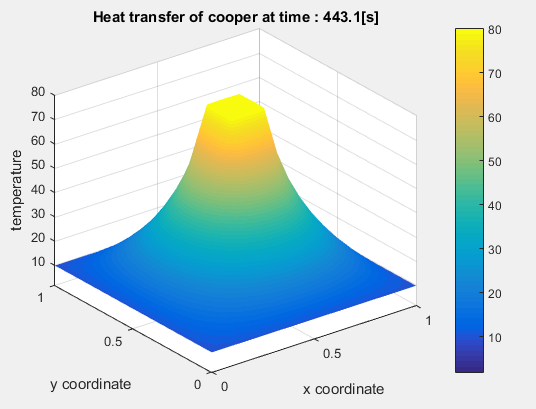
\includegraphics[scale=0.55]{1_cooper}
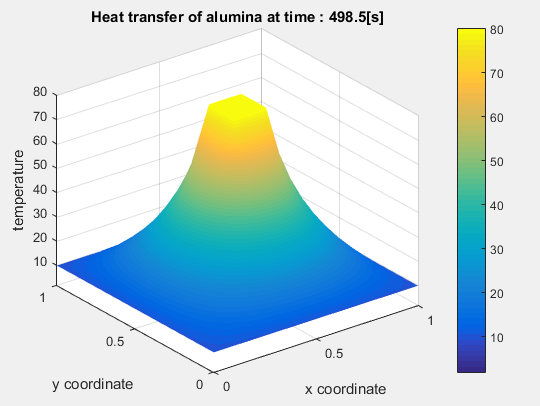
\includegraphics[scale=0.55]{1_alumina}
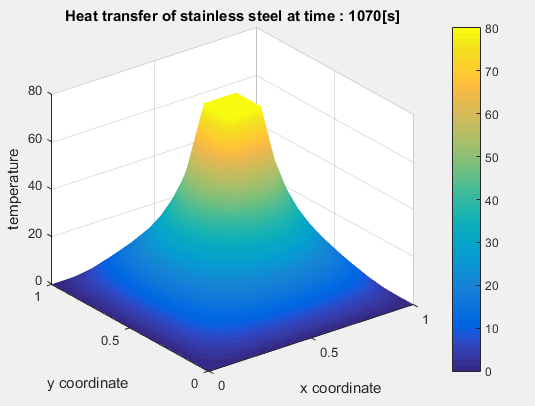
\includegraphics[scale=0.55]{1_steel}
\caption{Simulation states at the time of stabilization for different materials}
\centering
\end{figure}
Comparing plots we can  observe that time needed for stabilization was the highest for stainless steel material. It means that heat propagation in this material is the worst among 3 materials used in simulation. On the other hand cooper's heat propagation is the best, but only little better than alumina.
\section{Boundary Condition 2}
This boundary bondition assumes that heater works only for first 10 seconds and then shutdown. Power of heater is constant and equal $100[W]$. What is more, edges are thermally isolated from the environment. Temperature on the whole plate is $20[C]$.

\begin{figure}[H]
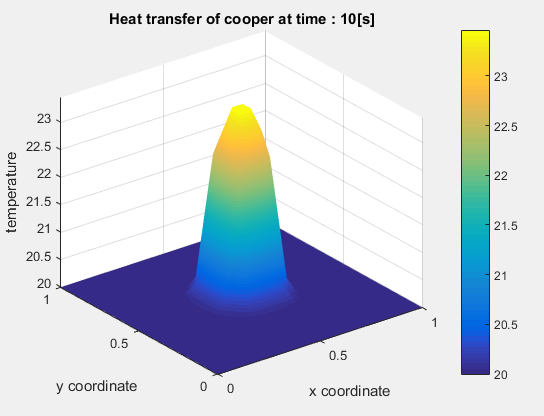
\includegraphics[scale=0.55]{2_cooper_heater_stop}
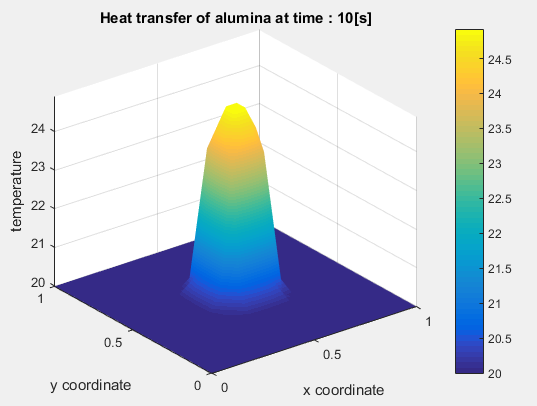
\includegraphics[scale=0.55]{2_alumina_heater_stop}
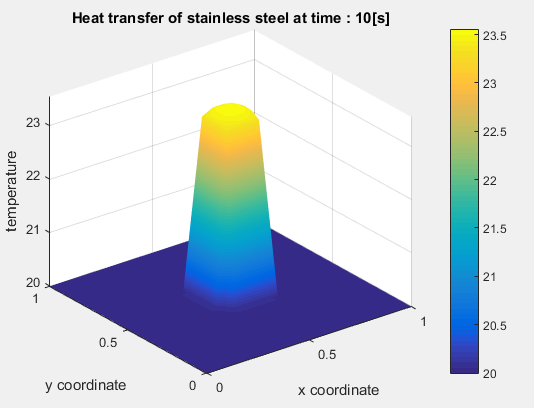
\includegraphics[scale=0.55]{2_steel_heater_stop}
\caption{Simulation states at the time of heater shutdown for different materials}
\centering
\end{figure}
In this figure we can observe how material reacts during heating.
\begin{figure}[H]
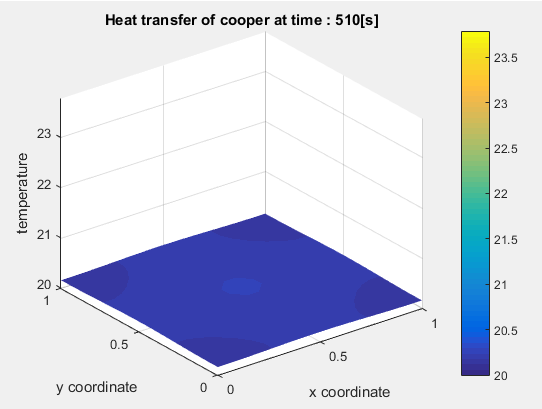
\includegraphics[scale=0.55]{2_cooper}
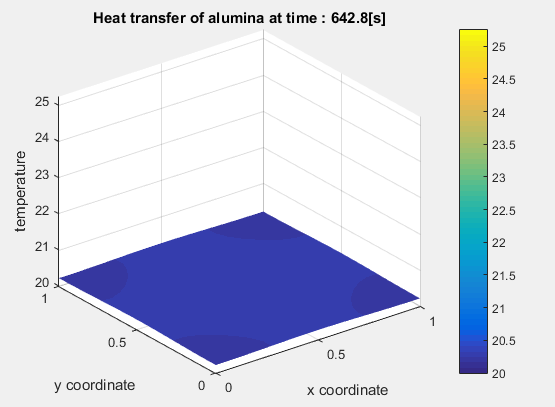
\includegraphics[scale=0.55]{2_alumina}
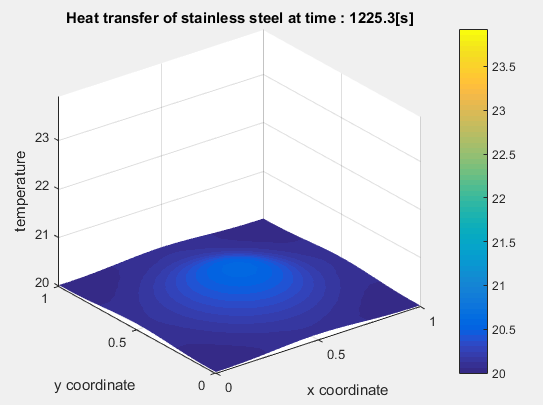
\includegraphics[scale=0.55]{2_steel}
\caption{Simulation states at the time of stabilization for different materials}
\centering
\end{figure}
Here we can see how much time is needed for uniform heat distribution on the plate for specific material. Results could be better if the acceptable error was smaller, but then time needed for stabilization would be greater. As we could assume the worst material for heat distribution is stainless steel. 

This plots also show how much even temperature of the plate will grow. Unfortunatelly, for used set of data change is very small ($\Delta T \approx 0.176$) so it is barely noticeable.
\subsection{Comparison with theorethical temperature change}
The heat delivered during heating is expressed by the following equation
\begin{equation*}
Q = c_w*m*\Delta T
\end{equation*}
where:
\begin{itemize}
\item $Q$ - Heat
\item $c_w$ - specific heat of the plate material
\item $\Delta T$ - difference in heat
\end{itemize}
We want to know how much temperature changed so we need to calculate $\Delta T$
\begin{equation*}
\Delta T = \frac{Q}{C_w*m} 
\end{equation*}
substituting $Q = P*t$ and $m = A^2*h*\rho$ we get 
\begin{equation*}
\Delta T = \frac{P*t}{C_w*A^2*h*\rho}
\end{equation*}
where:
\begin{itemize}
\item $P$ - power of the heater
\item $A^2$ - plate area
\item $h$ - plate thickness
\item $\rho$ - plate's material density
\end{itemize}
Using the data used in simulation for cooper we can calculate theoretical value of $\Delta T$
\begin{itemize}
\item $P = 100[W]$
\item $t = 10[s]$
\item $C_w = 380[\frac{J}{Kg*C}]$
\item $A = 1[m]$ - plate area
\item $h = 0.002[m]$ - plate thickness
\item $\rho = 8920[\frac{Kg}{m^3}]$ - plate's material density
\end{itemize}
The result is
\begin{equation*}
\Delta T \approx 0.148[C]
\end{equation*}
Adding $\Delta T$ to initial plate's temperature $T_0=20$ and comparing to simulation result $T_0 + \Delta T_{sim}=20.176$ we can say that values are not the same because of numerical errors and choosen precision for stopping the simulation. What is more calculating it by simulation is much more time consuming, however, sometimes for more complex situations, simulation seems to be the best way of calculating.Difference in values is acceptable.
\section{Numerical stability}
For the simulation presented in the figure below, I have used alumina material, $\delta t=0.4$ , $\delta x=0.01$. It is easy to observe that it is not acceptable result, it is coused by used equastion which for this values is not stable.
\begin{figure}[H]
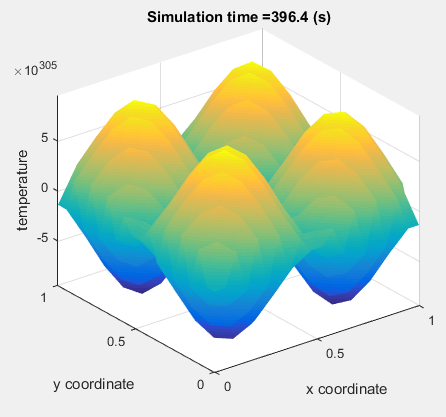
\includegraphics[scale=0.9]{numerical_stability}
\caption{Numerical oscilation}
\centering
\end{figure}

\section{Conclusions}
We have simulated heat transfer on the plate. It is great way to see how it changes in time. This is a big advantage. What is more as it was proved, it is possible to get results very similar to theoretical calculations.
We also observed how plate's material matters, and how different values can be. 
\newpage
\section{Source code}
Code is divided into sections responsible for data, first boundary , second boundary, numerical stability. What is more I extracted functions into another files which also are attached.\\
\lstinputlisting{lab3.m}
\lstinputlisting{deltaT_heater_equastion.m}
\lstinputlisting{equastion_fraction.m} 
\lstinputlisting{display_last_step.m}
\lstinputlisting{display_simulation.m}


\end{document}